%%This is a very basic article template.
%%There is just one section and two subsections.
\documentclass[11pt]{book}

% ***********************************************************
% ******************* PHYSICS HEADER ************************
% ***********************************************************
% Version 2

\usepackage{amsmath} % AMS Math Package
\usepackage{amsthm} % Theorem Formatting
\usepackage{amssymb}	% Math symbols such as \mathbb
\usepackage{graphicx} % Allows for eps images
\usepackage{multicol} % Allows for multiple columns
\usepackage[dvips,showframe,letterpaper,margin=1.0in,left=1.5in]{geometry}
% tim included
\usepackage[pdftex,bookmarks=true]{hyperref}

\usepackage{cancel}
\usepackage{siunitx}
 % Sets margins and page size
\pagestyle{plain} % Removes page numbers
\makeatletter % Need for anything that contains an @ command 
\renewcommand{\maketitle} % Redefine maketitle to conserve space
{ \begingroup \vskip 10pt \begin{center} \large {\bf \@title}
	\vskip 10pt \large \@author \hskip 20pt \@date \end{center}
  \vskip 10pt \endgroup \setcounter{footnote}{0} }
\makeatother % End of region containing @ commands
\renewcommand{\labelenumi}{(\alph{enumi})} % Use letters for enumerate
% \DeclareMathOperator{\Sample}{Sample}
\let\vaccent=\v % rename builtin command \v{} to \vaccent{}
\renewcommand{\v}[1]{\ensuremath{\mathbf{#1}}} % for vectors
\newcommand{\gv}[1]{\ensuremath{\mbox{\boldmath$ #1 $}}} 
% for vectors of Greek letters
\newcommand{\uv}[1]{\ensuremath{\mathbf{\hat{#1}}}} % for unit vector
\newcommand{\abs}[1]{\left| #1 \right|} % for absolute value
\newcommand{\avg}[1]{\left< #1 \right>} % for average
\let\underdot=\d % rename builtin command \d{} to \underdot{}
\renewcommand{\d}[2]{\frac{d #1}{d #2}} % for derivatives
\newcommand{\dd}[2]{\frac{d^2 #1}{d #2^2}} % for double derivatives
\newcommand{\pd}[2]{\frac{\partial #1}{\partial #2}} 
% for partial derivatives
\newcommand{\pdd}[2]{\frac{\partial^2 #1}{\partial #2^2}} 
% for double partial derivatives
\newcommand{\pdc}[3]{\left( \frac{\partial #1}{\partial #2}
 \right)_{#3}} % for thermodynamic partial derivatives
\newcommand{\ket}[1]{\left| #1 \right>} % for Dirac bras
\newcommand{\bra}[1]{\left< #1 \right|} % for Dirac kets
\newcommand{\braket}[2]{\left< #1 \vphantom{#2} \right|
 \left. #2 \vphantom{#1} \right>} % for Dirac brackets
\newcommand{\matrixel}[3]{\left< #1 \vphantom{#2#3} \right|
 #2 \left| #3 \vphantom{#1#2} \right>} % for Dirac matrix elements
\newcommand{\grad}[1]{\gv{\nabla} #1} % for gradient
\let\divsymb=\div % rename builtin command \div to \divsymb
\renewcommand{\div}[1]{\gv{\nabla} \cdot #1} % for divergence
\newcommand{\curl}[1]{\gv{\nabla} \times #1} % for curl
\let\baraccent=\= % rename builtin command \= to \baraccent
\renewcommand{\=}[1]{\stackrel{#1}{=}} % for putting numbers above =
\newtheorem{prop}{Proposition}
\newtheorem{thm}{Theorem}[section]
\newtheorem{lem}[thm]{Lemma}
\theoremstyle{definition}
\newtheorem{dfn}{Definition}
\theoremstyle{remark}
\newtheorem*{rmk}{Remark}

% ***********************************************************
% ********************** END HEADER *************************
% ***********************************************************
\pagenumbering{arabic}
\numberwithin{equation}{section}
%NEW COMMANDS
\newcommand{\beqa}{\begin{eqnarray*} }
\newcommand{\eeqa}{\end{eqnarray*} }
\newcommand{\beq}{\begin{equation} }
\newcommand{\eeq}{\end{equation} }
\newcommand{\beqB}{\begin{equation*}}
\newcommand{\eeqB}{\end{equation*}}

\newcommand{\beqaL}{\begin{eqnarray} }
\newcommand{\eeqaL}{\end{eqnarray} }
% macros used for consistency
\newcommand{\Psibar}{\bar{\Psi}}
\newcommand{\rapidity}{\phi}
\newcommand{\TensBi}{\Sigma} %(Tensor bilinear)

%nonrelativistic wave functions
\newcommand{\phis}{\phi_S}
\newcommand{\wnr}{\phi_S}
\newcommand{\wnrb}{\phi_S^\dagger}

%nonrelativistic fields
\newcommand{\fnr}{\Psi}
\newcommand{\fnrb}{\Psi^\dagger}

%relativistic fields
\newcommand{\fr}{\Psi}
\newcommand{\frb}{\bar{\Psi} }

%spinors u, ubar
\newcommand{\sr}{u}
\newcommand{\srb}{\bar{u}}

%General spin bispinor:
\newcommand{\Psig}{\Upsilon}
\newcommand{\Psigbar}{\bar{\Psig}}


\newcommand{\smalldot}{\cdot}
%from dirac_redo.tex
\newcommand{\sigdot}[1]{ \gv{\sigma} \hspace{-2pt} \cdot \hspace{-2pt} \v{#1} \,}
\newcommand{\sigdotg}[1]{ \gv{\sigma} \hspace{-2pt} \cdot \hspace{-2pt} \gv{#1} \,}
\newcommand{\explus}{(\sigdotg{\pi} - i\mu' \sigdot{E} )}
\newcommand{\exminus}{(\sigdotg{\pi} + i\mu' \sigdot{E} )}

\newcommand{\gradE}{\grad}

%Macro for weight matrix
\newcommand{\weight}{\Omega}


%matrix/vector/spinor shorthands
\newcommand{\spinor}[2]{ \begin{pmatrix} #1 \\ #2 \end{pmatrix} }
\newcommand{\Mblock}[4]{\begin{pmatrix} #1 & #2 \\ #3 & #4 \end{pmatrix} }

\newcommand{\Sb}{\overline{S}}

\newcommand{\A}{\epsilon}
\newcommand{\Adag}{\epsilon'}
\newcommand{\W}{\omega}
\newcommand{\Wdag}{\omega^*}

%-------
%macros for different term labels
%-------

%g dependent part of one photon calc
\newcommand{\Mg}{M_g}
%other part of one-photon calc
\newcommand{\Mq}{M_q}
%two-photon vertex contribution to Compton
\newcommand{\Mcontact}{M_{\text{contact}}}
\newcommand{\Mtrees}{M_{\text{trees} }}


\newcommand{\VertexEq}[2]{ \mbox{
\begin{minipage}{1.6in}
   \includegraphics[scale=0.8]{eps/#1} 
\end{minipage}
{ \large $	=	\hspace{2em} 	\large{#2} $ }
} }



% shortcuts for the binspinors represented as vectors.  Used in spin-half.tex, imported from uv_bilinears.tex
\newcommand{\uvec}[1]{ \begin{pmatrix} \varphi \\ \frac{\sigdot{#1}}{2m} \varphi \end{pmatrix} }
\newcommand{\vvec}[1]{ \begin{pmatrix} \frac{\sigdot{#1}}{2m} \chi \\ \chi \end{pmatrix} }
\newcommand{\udaggervec}[1]{ \begin{pmatrix} \varphi^\dagger & \frac{\sigdot{#1}}{2m} \varphi^\dagger \end{pmatrix} }
\newcommand{\vdaggervec}[1]{ \begin{pmatrix} \frac{\sigdot{#1}}{2m}  \chi^\dagger & \chi^\dagger \end{pmatrix} }

\newcommand{\ubar}{\bar{u}}
\newcommand{\vbar}{\bar{v}}%


%% Commands from spin1-diagrams
\newcommand{\snote}[1]{}
\newcommand{\qp}{q^{(+)}{}}
\newcommand{\qm}{q^{(-)}{}}
 \newcommand{\E}[1]{ \sqrt{ m^2 + \v{#1}^2 } }
% % \newcommand{\E}[1]{ E_{#1} }
 \newcommand{\diracdelta}[1]{ \delta^{(3)}(#1) }
 \newcommand{\epin}[1]{ \epsilon_{#1}(p) }
 \newcommand{\epout}[1]{ \epsilon^*_{#1}(p') }
\newcommand{\omin}[1]{ \omega_{#1}(p) }
 \newcommand{\omout}[1]{ \omega^*_{#1}(p') }


\usepackage{setspace}
\doublespacing
\begin{document}
\chapter{The interaction potential and final Hamiltonian}

\section{Calculation of Breit potential}
We want to calculate the interaction potential between two charged particles, at next to leading order.  We derive this potential from the one-photon exchange.
%TODO discuss exact path of derivation
We already have a Lagrangian for general-spin NRQED that is accurate to the order needed.  From this we can obtain the one photon vertex.  Working in the Coulomb gauge, the photon propagator is such that $D_{0i}=0$.  So we can think of it as splitting into two parts: represent $D_{00}$ by a dashed line, and $D_{ij}$ by a wavy one.  Then terms with $A_0$ and $A_i$ represent two types of vertices.

\subsection{Feynman rules}
The Coulomb vertex comes from the terms out of the general NRQED Lagrangian involving $A_0$:
\small
\beq
 \mathcal{L}_{A_0} =  \Psi^\dagger \Big (  -eA_0 
		+ c_D \frac{ e(\v{\grad} \smalldot \v{E} - \v{E} \smalldot \v{\grad} ) }{8m^2}	
		+ c_Q \frac{e Q_{ij} (\nabla_i E_j - E_i \nabla_j) }{8m^2}	
		+ c^{1}_S \frac{ ie \v{S} \smalldot ( \v{\grad} \times \v{E} - \v{E} \times \v{\grad} )}{8m^2}
		\Big )\Psi
\eeq
\normalsize
%Term by term 

\mbox{
\begin{minipage}{1.2in}
   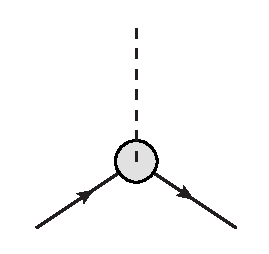
\includegraphics[scale=0.7]{eps/DashVertexNRQED} 
\end{minipage}
 = \hspace{.5em} $V_0 $ \hspace{.5em} 
 = \hspace{.5em} $ i e \Big ( 1 + \frac{1}{8m^2} \big [  c_D \v{q}^2 + c_Q Q_{ij} q_i q_j - 2 i c_S \v{S} \cdot \v{p} \times \v{q} \big ]\Big)$
}



The  part of the Lagrangian representing interaction with a transverse photon is
\beqa
\mathcal{L}_{\v{A}} &=& \Psi^\dagger \big (  - ie  \frac{ \{\nabla_i, A_i \} }{2m} 
		+ c_F e \frac{\v{S} \smalldot \v{B}} {2m}   	
		\big )\Psi
\eeqa


So the transverse vertex is

\mbox{
\begin{minipage}{1.4in}
   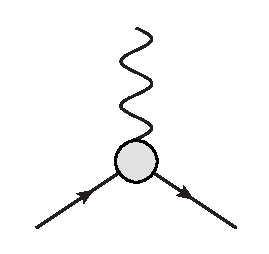
\includegraphics[scale=0.7]{eps/WaveVertexNRQED} 
\end{minipage}
 = \hspace{1em} $V_i $ \hspace{1em} 
 = \hspace{1em} $ i\frac{e}{2m} \Big ( \v{p} + \v{p'} + c_F i \v{S} \times \v{q} \Big)_i$
}


\subsection{Calculation of interaction}


The two particles will have Lagrangians, and thus vertices, of the same general form.  However, the coefficients will differ, so denote the coefficients of the second particle by $d$ rather than $c$.  Call the particles $1$ and $2$, and denote which field operators act on with these numerals.  Then the interaction diagrams will be

%
%%   Dashed diagram
%%%
%%%%%%%%%%%%%%%%%%%%
\mbox{
\begin{minipage}{1in}
   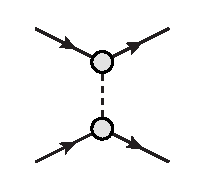
\includegraphics[scale=0.7]{eps/DashBreit} 
\end{minipage}
 = \hspace{0.5em} $V^1_0 V^2_0  D_{00} $ \hspace{1em} 
 = \hspace{0.5em} 

\begin{minipage}{4in} %Equation for dashed breit
\small
\beq
\begin{split}
	\left[ -\frac{1}{\v{q}^2} \right]  
	ie_2\phi_2^\dagger \left\{  1 - \frac{1}{8m_2^2}\left ( d_D \v{q}^2  + d_Q {Q_2}_{ij} q_i q_j + 2 i d_S \v{S}_2 \cdot \v{p}_2 \times \v{q} \right ) \right \}\phi_2	 
\\	\times \hspace{1em} ie_1\phi_1^\dagger \left\{  1 - \frac{1}{8m_1^2}\left ( c_D \v{q}^2 + c_Q {Q_1}_{ij} q_i q_j - 2 i c_S \v{S}_1 \cdot \v{p}_1 \times \v{q}   \right ) \right \}\phi_1	 
\end{split}
\eeq
\normalsize
\end{minipage}
}

The expansion to the order needed is trivial:
\beq \begin{split}
V^1_0 V^2_0  D_{00} = e_1 e_2 \frac{1}{\v{q}^2} (\phi^\dagger_1 \phi^\dagger_2 \phi_2 \phi_1) \Big [
	1 - \frac{1}{8m_2^2}\left ( d_D \v{q}^2  + d_Q {Q_2}_{ij} q_i q_j + 2 i c_S \v{S}_2 \cdot \v{p}_2 \times \v{q} \right ) 
	\\  - \frac{1}{8m_1^2}\left ( c_D \v{q}^2 + c_Q {Q_1}_{ij} q_i q_j - 2 i c_S \v{S}_1 \cdot \v{p}_1 \times \v{q}   \right )
\Big ] 
\end{split}
\eeq




%%
%%  Wavey diagram
%%
%%%%%%%%%%%%%%%%%%%%
The exchange of a transverse photon is given by

\mbox{
\begin{minipage}{1in}
   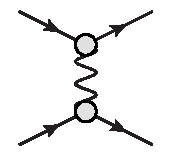
\includegraphics[scale=0.7]{eps/WaveBreit} 
\end{minipage}
 = \hspace{0.5em} $V^1_i V^2_j  D_{ij} $ \hspace{1em} 
 = \hspace{0.5em} 

\begin{minipage}{1.4in} %equation for Wavey breit
\small
\[
	\left[ \frac{i e_1}{2m_1} \phi_1^\dagger \left\{ (2p_1 + q)^i - c_F i\epsilon_{k\ell i} q_k {S_1}_\ell \right \} \phi_1 \right ]
	\left[ \frac{1}{\v{q}^2} \left(\delta_{ij} - \frac{q_i q_j}{\v{q}^2} \right ) \right ]
\]
\[
	\times \left[ \frac{i e_2}{2m_2} \phi_2^\dagger \left\{ (2p_2 - q)^j + d_F i\epsilon_{m n j} q_m {S_2}_n \right \} \phi_1 \right ]
\]
\normalsize
\end{minipage}
}


This is a mess of terms that will simplify.  Consider first the inner terms with just $\delta_{ij}$.  Some terms drop out because $q_i q_j \epsilon_{ijk}=0$.
\beq
\delta_{ij} \left[ (2p_1 + q)^i - i c_F (\epsilon_{k\ell i} q_k {S_1}_\ell)   \right ]	
	\left[  (2p_2 - q)^j + i d_F (\epsilon_{m n j} q_m {S_2}_n)  \right ]
\eeq
\beq
\begin{split}
 	=& (2\v{p_1} + \v{q}) \cdot ( 2\v{p_2} - \v{q}) + 2 i  d_F q_m {S_2}_n p_j \epsilon_{mnj} - 2 i c_F q_k{S_1}_\ell p_k \epsilon_{k\ell i} ) 
 	\\&+ (c_F d_F) q_k q_m {S_1}_\ell {S_2}_n (\delta_{km} \delta_{\ell n } - \delta_{kn} \delta_{\ell m} )
\\	=& (2\v{p_1} + \v{q}) \cdot ( 2\v{p_2} - \v{q}) + 2i \v{q} \cdot ( d_F \v{S_2} \times \v{p_1} - c_F \v{S_1} \times \v{p_2} ) 
	\\& + c_F d_F \big(\v{q}^2 \v{S_1} \cdot \v{S_2} - (\v{S_1} \cdot \v{q})(\v{S_2} \cdot \v{q})\big)
\end{split}
\eeq

Now consider the contraction with $q_i q_j$.  This is much simpler, as $\v{q} \times \v{q}=0$.
\[
q_i q_j \left[ (2p_1 + q)^i - i c_F \epsilon_{k\ell i} q_k {S_1}_\ell   \right ]	
	\left[  (2p_2 - q)^j + i d_F \epsilon_{m n j} q_m {S_2}_n  \right ]
\]
\[
	=	(2 \v{p_1} + \v{q}) \cdot \v{q} (2\v{p_2} - \v{q}) \cdot \v{q} 
	=      4 (\v{p_1} \cdot \v{q})( \v{p_2} \cdot \v{q}) + \v{q}^2 ( 2\v{p_2} \cdot \v{q} - 2\v{p_1} \cdot \v{q} - \v{q}^2 )
\]

So 

\mbox{
\begin{minipage}{0.8in}
   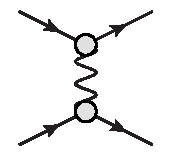
\includegraphics[scale=0.7]{eps/WaveBreit} 
\end{minipage}
 = \hspace{0.5em} \scriptsize{ $V^1_i V^2_j  D_{ij} $}\hspace{0.5em} 
 = 
\begin{minipage}{4in} %equation for Wavey breit
\scriptsize
\beq
\begin{split} & -\frac{ e_1 e_2 }{4 m_1 m_2} \frac{1}{\v{q}^2} (\phi^\dagger_1 \phi^\dagger_2 \phi_2 \phi_1)
\Bigg \{	
	4\left( \v{p_1} \cdot \v{p_2} - \frac{(\v{p_1} \cdot \v{q})( \v{p_2} \cdot \v{q})}{\v{q}^2} \right )
\\& + 2i \v{q} \cdot ( d_F \v{S_2} \times \v{p_1} - c_F \v{S_1} \times \v{p_2} )
	+ c_F d_F \big(\v{q}^2 \v{S_1} \cdot \v{S_2} - (\v{S_1} \cdot \v{q})(\v{S_2} \cdot \v{q})\big)
\Bigg \} 
\end{split}
\eeq
\normalsize
\end{minipage}
}




The total interaction is then

\beqa
M &=& e_1 e_2 \frac{1}{\v{q}^2} (\phi^\dagger_1 \phi^\dagger_2 \phi_2 \phi_1) \Big\{
	1 - \frac{1}{8m_2^2}\left ( d_D \v{q}^2  + d_Q {Q_2}_{ij} q_i q_j + 2 i d_S \v{S}_2 \cdot \v{p}_2 \times \v{q} \right ) 
 \\&&	- \frac{1}{8m_1^2}\left ( c_D \v{q}^2 + c_Q {Q_1}_{ij} q_i q_j - 2 i c_S \v{S}_1 \cdot \v{p}_1 \times \v{q}   \right )
	- \frac{1}{m_1 m_2}\left( \v{p_1} \cdot \v{p_2} - \frac{(\v{p_1} \cdot \v{q})( \v{p_2} \cdot \v{q})}{\v{q}^2} \right )
\\&&	- \frac{i }{2 m_1 m_2} \v{q} \cdot ( d_F \v{S_2} \times \v{p_1} - c_F \v{S_1} \times \v{p_2} )
	- \frac{c_F d_F}{4 m_1 m_2} \big(\v{q}^2 \v{S_1} \cdot \v{S_2} - (\v{S_1} \cdot \v{q})(\v{S_2} \cdot \v{q})\big)
	\Big \}
\eeqa
If we distribute the $1/\v{q}^2$ we get


\beqa
M &=& e_1 e_2 (\phi^\dagger_1 \phi^\dagger_2 \phi_2 \phi_1) \Big\{
	\frac{1}{\v{q}^2} - \frac{1}{8m_2^2}\left ( d_D   + d_Q {Q_2}_{ij} \frac{  q_i q_j }{\v{q}^2 } + 2 i d_S \frac{\v{q} \cdot \v{S_2} \times \v{p_2} }{\v{q}^2}  \right ) 
\\&&	- \frac{1}{8m_1^2}\left ( c_D   + c_Q {Q_1}_{ij} \frac{ q_i q_j }{\v{q}^2 } - 2 i c_S \frac{\v{q} \cdot \v{S_1} \times \v{p_1} }{\v{q}^2}  \right ) 
	-  \frac{1}{m_1 m_2}\left( \frac{\v{p_1} \cdot \v{p_2}}{\v{q}^2} - \frac{(\v{p_1} \cdot \v{q})( \v{p_2} \cdot \v{q})}{\v{q}^4} \right )
\\&&	- \frac{i }{2 m_1 m_2} \frac{\v{q} \cdot ( d_F \v{S_2} \times \v{p_1} - c_F \v{S_1} \times \v{p_2} )}{\v{q}^2}
	- \frac{c_F d_F}{4 m_1 m_2} \big( \v{S_1} \cdot \v{S_2} - \frac{(\v{S_1} \cdot \v{q})(\v{S_2} \cdot \v{q})}{\v{q}^2}\big)
	\Big \}
\eeqa



\subsection{Position space potential}

Define $U(\v{p_1}, \v{p_2}, \v{q})$ by 
\[
	M = (\phi^\dagger_1 \phi^\dagger_2 \phi_2 \phi_1) U(\v{p_1}, \v{p_2}, \v{q})
\] so
\beq \begin{split}
	U(\v{p_1}, \v{p_2}, \v{q}) =& 	 e_1 e_2   \Big\{
	\frac{1}{\v{q}^2} - \frac{1}{8m_2^2}\left ( d_D   + d_Q {Q_2}_{ij} \frac{  q_i q_j }{\v{q}^2 } + 2 i d_S \frac{\v{q} \cdot \v{S_2} \times \v{p_2} }{\v{q}^2}  \right ) 
\\&	- \frac{1}{8m_1^2}\left ( c_D   + c_Q {Q_1}_{ij} \frac{ q_i q_j }{\v{q}^2 } - 2 i c_S \frac{\v{q} \cdot \v{S_1} \times \v{p_1} }{\v{q}^2}  \right ) 
	-  \frac{1}{m_1 m_2}\left( \frac{\v{p_1} \cdot \v{p_2}}{\v{q}^2} - \frac{(\v{p_1} \cdot \v{q})( \v{p_2} \cdot \v{q})}{\v{q}^4} \right )
\\&	- \frac{i }{2 m_1 m_2} \frac{\v{q} \cdot ( d_F \v{S_2} \times \v{p_1} - c_F \v{S_1} \times \v{p_2} )}{\v{q}^2}
	- \frac{c_F d_F}{4 m_1 m_2} \big( \v{S_1} \cdot \v{S_2} - \frac{(\v{S_1} \cdot \v{q})(\v{S_2} \cdot \v{q})}{\v{q}^2}\big)
	\Big \}
\end{split}\eeq

We want to transform this expression into position space.  Opening up Berestetskii/Pitaevskii we have the following transformations.

\beqa
	\int e^{i \v{q} \cdot \v{r} } \frac{d^3q}{(2\pi)^3} 
		&=& \delta^{(3)}(\v{r})	\\
	\int e^{i \v{q} \cdot \v{r} } \frac{d^3q}{(2\pi)^3} \frac{1}{\v{q}^2} 
		&=& \frac{1}{4\pi r}	\\
	\int e^{i \v{q} \cdot \v{r} } \frac{d^3q}{(2\pi)^3} \frac{q_i}{\v{q}^2} 
		&=& \frac{i r_i}{4\pi r^3}	\\
	\int e^{i \v{q} \cdot \v{r} } \frac{d^3q}{(2\pi)^3} \frac{q_i q_j}{\v{q}^4} 
		&=& \frac{1}{8\pi r} \left(  \delta_{ij} - \frac{r_i r_j}{r^2}  \right )	\\	
	\int e^{i \v{q} \cdot \v{r} } \frac{d^3q}{(2\pi)^3} \frac{q_i q_j}{\v{q}^2} 
		&=& \frac{1}{4\pi r^3} \left(  \delta_{ij} - 3\frac{r_i r_j}{r^2}  \right ) + \frac{1}{3} \delta_{ij} \delta^{(3)}(\v{r})	\\	
\eeqa

The quadrupole moment $Q_{ij}$ is symmetric and traceless.  This means
\[
	Q_{ij} (\delta_{ij} - 3\frac{r_i r_j}{r^2}) = - 3 \frac{Q_{ij} r_i r_j}{r^2}
\]



Now applying the identities above, we find the Fourier transform of $U$.

\small
\beq
\begin{split}
	\overline{U}(\v{p_1}, \v{p_2}, \v{r}) =& 	
	 e_1 e_2 \Bigg[ 
		\frac{1}{4\pi r} 
		- \frac{1}{8m_2^2}\left ( d_D \delta(\v{r})  - 3 d_Q \frac{{Q_2}_{ij} r_i r_j}{4 \pi r^5}   - d_S \frac{\v{r} \cdot \v{S_2} \times \v{p_2} }{2\pi r^3}   \right )
 	\\&	- \frac{1}{8m_1^2}\left ( \delta(\v{r}) - 3 c_Q \frac{{Q_1}_{ij} r_i r_j}{4 \pi r^5}  + c_S \frac{\v{r} \cdot \v{S_1} \times \v{p_1} }{2\pi r^3}   \right )
	\\&	- \frac{1}{m_1 m_2}\left( \frac{\v{p_1} \cdot \v{p_2}}{4\pi r} - \frac{1}{8 \pi r}\left\{ \v{p_1} \cdot \v{p_2} - \frac{(\v{p_1} \cdot \v{r}) (\v{p_2} \cdot \v{r}) }{r^2} \right\} \right )
	\\&	+ \frac{1}{2 m_1 m_2} \frac{  \v{r} \cdot ( d_F \v{S_2} \times \v{p_1} - c_F \v{S_1} \times \v{p_2} )}{4\pi r^3}
	\\&	- \frac{c_F d_F }{4 m_1 m_2}\bigg( \v{S_1} \cdot \v{S_2} \delta(\v{r}) 
			- \frac{1}{4\pi r^3} \left\{ \v{S_1} \cdot \v{S_2} - 3 \frac{(\v{S_1} \cdot \v{r}) (\v{S_2} \cdot \v{r}) }{r^2}\right \}
			- \v{S_1} \cdot \v{S_2} \frac{1}{3} \delta(\v{r})   \bigg)
	\Bigg]
\end{split}	
\eeq
\normalsize

Or combining the few like terms

\small
\beqa
	\overline{U}(\v{p_1}, \v{p_2}, \v{r}) &=& 	
	 e_1 e_2 \Bigg[ 
		\frac{1}{4\pi r} 
		- \frac{1}{8m_2^2}\left ( d_D \delta(\v{r})  - 3 d_Q \frac{{Q_2}_{ij} r_i r_j}{4 \pi r^5}   - d_S \frac{\v{r} \cdot \v{S_2} \times \v{p_2} }{2\pi r^3}   \right )
 	\\&&	- \frac{1}{8m_1^2}\left ( c_D \delta(\v{r}) - 3 c_Q \frac{{Q_1}_{ij} r_i r_j}{4 \pi r^5}  + c_S \frac{\v{r} \cdot \v{S_1} \times \v{p_1} }{2\pi r^3}   \right )
	\\&&	- \frac{1}{m_1 m_2}\left( \frac{\v{p_1} \cdot \v{p_2}}{8\pi r} + \frac{(\v{p_1} \cdot \v{r}) (\v{p_2} \cdot \v{r}) }{8 \pi r^3}  \right ) 
	\\&&	+ \frac{1}{2 m_1 m_2} \frac{ \v{r} \cdot ( d_F \v{S_2} \times \v{p_1} - c_F \v{S_1} \times \v{p_2} )}{4\pi r^3}
	\\&&	- \frac{c_F d_F }{4 m_1 m_2}\bigg( \frac{2}{3} \v{S_1} \cdot \v{S_2} \delta(\v{r}) 
			- \frac{1}{4\pi r^3} \left\{ \v{S_1} \cdot \v{S_2} - 3 \frac{(\v{S_1} \cdot \v{r}) (\v{S_2} \cdot \v{r}) }{r^2}  \right \}  \bigg)
	\Bigg]
\eeqa
\normalsize

This represents the interaction in the absence of any external magnetic field.  However, to derive the $g$-factor that is exactly the needed interaction.  These additional terms will come from diagrams which involve both the exchange of a photon and interaction with the potential $\v{A}$.

\section{Photon exchange in an external field}

\subsection{Feynman rules}



We want to derive the interaction potential when there is an external magnetic field present.  We derive this from diagrams which involve not just the exchange of one photon, but also an additional interaction with the external field.

Because we consider the point-like interaction we don't need to consider diagrams which contain either charged-particle's propagator.  So the interaction we're interested in will necessarily involve two-photon vertices.  The part of the NRQED Lagrangian with such terms is:

\scriptsize
\beqa
	\mathcal{L}_{A^2} &=& \Psi^\dagger ( - \frac{e^2 \v{A}^2}{2m}  - e^2 \frac{ \{ \grad^2, \v{A}^2 \} 
}{8m^3} - e^2\frac{ \{\nabla_i, A_i \} \{\nabla_j, A_j\} }{8m^3}
		+ c_S \frac{ e^2 \v{S} \smalldot ( \v{A} \times \v{E} - \v{E} \times \v{A} )}{8m^2} ) \Psi
\eeqa
\normalsize


Organise the terms in the two-photon Lagrangian so that they look like:
\[
	\mathcal{L}_{A^2} = A_0 A_i \Psi^\dagger \Psi W_{i}(\v{p}, q) + A_i A_j \Psi^\dagger \Psi W_{ij}(\v{p}, q) + A_0 A_0 \Psi^\dagger \Psi W_0 
\]
It'll turn out we want only the very first leading order terms of $W_i$ and $W_{ij}$.  (These $W$ shouldn't be confused with the fields in the spin-one calculation.)  The leading order term in $W_{ij}$ is
\[
	W_{ij} = - \frac{e^2 \delta_{ij}}{2m}
\]	

The leading order term in $W_i$ comes from the $\v{A} \times \v{E}$ term.  $\v{E} = -\partial_0 \v{A} - \grad A_0$.  So
\[
	W_i = - i c_S \frac{e^2}{4m^2} \epsilon_{ijk} {q_j S_k} 
\]


From these we can write down the diagrams.  The vertex with two transverse photons carrying indices $i$ and $j$ is associated with a symmetry factor of $1/2$, so

\begin{center}
\mbox{
	\begin{minipage}{1in}
	   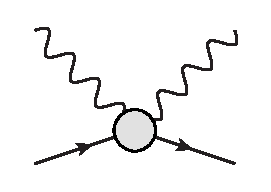
\includegraphics[scale=0.5]{eps/WaveWaveVertex} 
	\end{minipage}
	$ = 2 W_{ij} =  -i\frac{e^2 \delta_{ij}}{m} $
}
\end{center}

The vertex one transverse line (index $i$ and momentum $k$) and one Coulomb photon (incoming momentum $q$):

\begin{center}
\mbox{
	\begin{minipage}{1in}
	   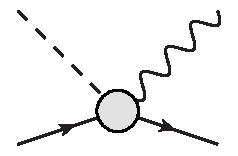
\includegraphics[scale=0.5]{eps/DashWaveVertex} 
	\end{minipage}
	$ = W_i  =  c_S \frac{e^2}{4m^2} \epsilon_{ijk} {q_j S_k} $
}
\end{center}
The external field $\v{A}$ will be contracted with such vertices; it will be necessary to label the external field just as it was necessary to label the particles.  The convention is that in position space $\v{A}_1 = \v{A}(\v{r}_1)$ and $\v{A}_2 = \v{A}(\v{r}_2)$. 

We also need the one-photon vertices which were derived in the previous section, but only to leading order.  These are, dropping those higher order terms:

\mbox{
	\begin{minipage}{1in}
	   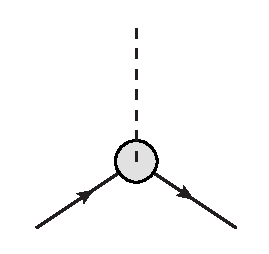
\includegraphics[scale=0.5]{eps/DashVertexNRQED} 
	\end{minipage}
	 = \hspace{1em} $ i e $
}
\hspace{5em}
\mbox{
	\begin{minipage}{1in}
	   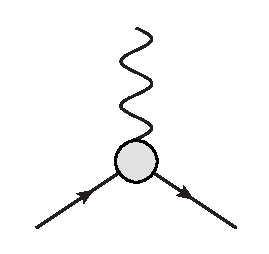
\includegraphics[scale=0.5]{eps/WaveVertexNRQED} 
	\end{minipage}
	 = \hspace{1em} $ i\frac{e}{2m} \Big ( \v{p} + \v{p'} + c_F i \v{S} \times \v{q} \Big)_i$
}

The Coulomb propagator is just as it was before.

\subsection{Interaction diagrams}

There are four diagrams that capture the type of interaction we're looking for.  The particles can exchanged either a transverse or Coulomb photon, and either particle can interact with the external magnetic field.  In each of the diagrams, let $q$ be the momentum of the exchanged photon, directed towards the vertex of particle one.  Let $k$ be the momenta of the photon interacting with the external field. 


First, the two diagrams with Coulomb exchange:

\mbox{
	\begin{minipage}{1in}
	   	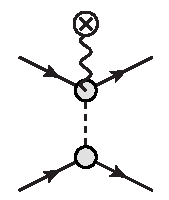
\includegraphics[scale=0.7]{eps/DashBreitA1} 
	\end{minipage}
	 = \hspace{1em} 
	$
	 	\phi^\dagger_2\Big(  ie_2  \Big )\phi_2
		\Big( - \frac{1}{\v{q}^2}	\Big )
		\phi^\dagger_1\Big(  c_S \frac{e_1^2}{4m_1^2} \v{S_1} \cdot \v{A}_1 \times \v{q}  \Big )\phi_1
	$
}

\[
	=	- i e_1 e_2 (\phi^\dagger_2 \phi^\dagger_1 \phi_1 \phi_2) c_s \frac{e_1}{4m_1^2} \frac{\v{S_1} \cdot \v{A}_1 \times \v{q} }{\v{q}^2}
\]


The diagram representing the second particle's interaction:

\mbox{
	\begin{minipage}{1in}
	   	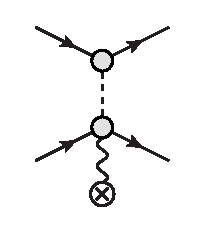
\includegraphics[scale=0.7]{eps/DashBreitA2} 
	\end{minipage}
	 = \hspace{1em} 
	\begin{minipage}{1in}
	\[
		-\phi^\dagger_2\Big(  d_S \frac{e_2^2}{4m_2^2} \v{S_2} \cdot \v{A}_2 \times \v{q}  \Big )\phi_2
	 	\Big( - \frac{1}{\v{q}^2}	\Big )
		\phi^\dagger_1\Big(  ie_1  \Big )\phi_1
	\]
	\end{minipage}
}

\[
	=	+ i e_1 e_2 (\phi^\dagger_2 \phi^\dagger_1 \phi_1 \phi_2) d_S \frac{e_2}{4m_2^2} \frac{\v{S_2} \cdot \v{A}_2 \times \v{q} }{\v{q}^2}
\]


Then, diagrams with transverse exchange:

\mbox{
	\begin{minipage}{1in}
	   	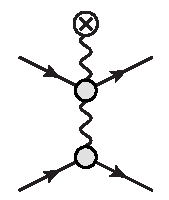
\includegraphics[scale=0.7]{eps/WaveBreitA1} 
	\end{minipage}
	 = \hspace{1em} 
	\begin{minipage}{1in}
	\[
		\phi_2^\dagger\Big(   i\frac{e_2}{2m_2} [2 p_2 - q - d_F i \v{S_2} \times \v{q}]_i  \Big )\phi_2
		\Big( \frac{\delta_{ij}}{\v{q}^2} - \frac{ q_i q_j}{\v{q}^4} \Big )
		\phi_1^\dagger\Big (  \frac{-i e_1^2 A_j }{m_1}\Big ) \phi_1 
	\]
	\end{minipage}
}

\beq
	=	e_1 e_2 (\phi^\dagger_2 \phi^\dagger_1 \phi_1 \phi_2) \frac{e_1}{2 m_1 m_2} \Big ( 
			\frac{ (2\v{p}_2 - \v{q}) \cdot \v{A}_1 }{\v{q}^2} 
			- i d_F \frac{ \v{S}_2 \cdot \v{q} \times \v{A}_1 }{\v{q}^2} 
			- \frac{ (2\v{p}_2 - \v{q}) \cdot \v{q} \v{A}_1 \cdot \v{q} }{\v{q}^4}
		\Big)
\eeq
\beq
	=	e_1 e_2 (\phi^\dagger_2 \phi^\dagger_1 \phi_1 \phi_2) \frac{e_1}{2 m_1 m_2} \Big ( 
			\frac{ 2\v{p}_2  \cdot \v{A}_1 }{\v{q}^2} 
			- i d_F \frac{ \v{S}_2 \cdot \v{q} \times \v{A}_1 }{\v{q}^2} 
			- \frac{ (2\v{p}_2 \cdot \v{q}) (\v{A}_1 \cdot \v{q}) }{\v{q}^4 }
		\Big)
\eeq



\mbox{
	\begin{minipage}{1in}
	   	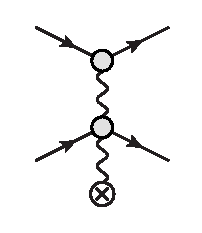
\includegraphics[scale=0.7]{eps/WaveBreitA2} 
	\end{minipage}
	 = \hspace{1em} 
	\begin{minipage}{1in}
	\[
		\phi_2^\dagger \Big ( \frac{-i e_2^2 A_j }{m_2} \Big )\phi_2 
		\Big( \frac{\delta_{ij}}{\v{q}^2} - \frac{ q_i q_j}{\v{q}^4} \Big )
		\phi_1^\dagger\Big(   i\frac{e_1}{2m_1} [2 p_1 + q + c_F i \v{S_1} \times \v{q}]_i \Big )\phi_1 
	\]
	\end{minipage}
}
\beq
	=	e_1 e_2 (\phi^\dagger_2 \phi^\dagger_1 \phi_1 \phi_2) \frac{e_2}{2 m_1 m_2} \Big ( 
			\frac{ (2\v{p}_1 + \v{q}) \cdot \v{A}_2 }{\v{q}^2} 
			+ i c_F \frac{ \v{S}_1 \cdot \v{q} \times \v{A}_2 }{\v{q}^2} 
			- \frac{ (2\v{p}_1 + \v{q}) \cdot \v{q} \v{A}_2 \cdot \v{q} }{\v{q}^4}
		\Big)
\eeq


\beq
	=	e_1 e_2 (\phi^\dagger_2 \phi^\dagger_1 \phi_1 \phi_2) \frac{e_2}{2 m_1 m_2} \Big ( 
			\frac{ 2\v{p}_1  \cdot \v{A}_2 }{\v{q}^2} 
			+ i c_F \frac{ \v{S}_1 \cdot \v{q} \times \v{A}_2 }{\v{q}^2} 
			- \frac{ (2\v{p}_1 \cdot \v{q}) (\v{A}_2 \cdot \v{q}) }{\v{q}^4 }
		\Big)
\eeq

The total contribution to the interaction potential from these diagrams would then be 
\beqa
U_2(\v{p_1}, \v{p_2}, \v{q}) &=& 	 e_1 e_2   \Big\{
	- i c_s \frac{e_1}{4m_1^2} \frac{\v{S_1} \cdot \v{A}_1 \times \v{q} }{\v{q}^2}
	+ i d_S \frac{e_2}{4m_2^2} \frac{\v{S_2} \cdot \v{A}_2 \times \v{q} }{\v{q}^2}
\\&&	+\frac{e_1}{ m_1 m_2} \Big ( 
		\frac{ \v{p}_2  \cdot \v{A}_1 }{\v{q}^2} 
		- i d_F \frac{ \v{S}_2 \cdot \v{q} \times \v{A}_1 }{2\v{q}^2} 
		- \frac{ (\v{p}_2 \cdot \v{q}) (\v{A}_1 \cdot \v{q}) }{\v{q}^4 }
	\Big )
\\&&	+\frac{e_2}{ m_1 m_2} \Big ( 
			\frac{ \v{p}_1  \cdot \v{A}_2 }{\v{q}^2} 
			+ i c_F \frac{ \v{S}_1 \cdot \v{q} \times \v{A}_2 }{2\v{q}^2} 
			- \frac{ (\v{p}_1 \cdot \v{q}) (\v{A}_2 \cdot \v{q}) }{\v{q}^4 }
	\Big)
\Big\}
\eeqa

None of these terms are gauge-invariant by themselves.  So we'd expect the above to agree with what we'd get if we took the terms in the potential without $\v{A}$ and restored gauge invariance.  That potential was:
\small
\beqa
	U_1(\v{p_1}, \v{p_2}, \v{q}) &=& 	 e_1 e_2   \Big\{
	\frac{1}{\v{q}^2} - \frac{1}{8m_2^2}\left ( d_D   + d_Q {Q_2}_{ij} \frac{  q_i q_j }{\v{q}^2 } + 2 i d_S \frac{\v{q} \cdot \v{S_2} \times \v{p_2} }{\v{q}^2}  \right ) 
\\&&	- \frac{1}{8m_1^2}\left ( c_D   + c_Q {Q_1}_{ij} \frac{ q_i q_j }{\v{q}^2 } - 2 i c_S \frac{\v{q} \cdot \v{S_1} \times \v{p_1} }{\v{q}^2}  \right ) 
	-  \frac{1}{m_1 m_2}\left( \frac{\v{p_1} \cdot \v{p_2}}{\v{q}^2} - \frac{(\v{p_1} \cdot \v{q})( \v{p_2} \cdot \v{q})}{\v{q}^4} \right )
\\&&	- \frac{i }{2 m_1 m_2} \frac{\v{q} \cdot ( d_F \v{S_2} \times \v{p_1} - c_F \v{S_1} \times \v{p_2} )}{\v{q}^2}
	- \frac{c_F d_F}{4 m_1 m_2} \big( \v{S_1} \cdot \v{S_2} - \frac{(\v{S_1} \cdot \v{q})(\v{S_2} \cdot \v{q})}{\v{q}^2}\big)
	\Big \}
\eeqa
\normalsize
Picking out only terms with the momentum operators $\v{p}_1$, $\v{p}_2$, which we'll call $U_p$, we find:
\beqa
	U_p(\v{p_1}, \v{p_2}, \v{q}) &=&  e_1 e_2   \Big\{
	\frac{1}{4m_1^2}\left (   i c_S \frac{\v{q} \cdot \v{S_1} \times \v{p_1} }{\v{q}^2}  \right ) 
	 - \frac{1}{4m_2^2}\left (  i d_S \frac{\v{q} \cdot \v{S_2} \times \v{p_2} }{\v{q}^2}  \right ) 
\\&&	-  \frac{1}{m_1 m_2}\left( \frac{\v{p_1} \cdot \v{p_2}}{\v{q}^2} - \frac{(\v{p_1} \cdot \v{q})( \v{p_2} \cdot \v{q})}{\v{q}^4} \right )
	- \frac{i }{2 m_1 m_2} \frac{\v{q} \cdot ( d_F \v{S_2} \times \v{p_1} - c_F \v{S_1} \times \v{p_2} )}{\v{q}^2}
	\Big \}
\eeqa
If we substitute $\v{p} \to \v{p} - e\v{A}$ we restore exactly (ignoring $A^2$ terms) the terms in $U_2$.  So the position space potential in the presence of this external field may also be obtained by just the procedure of minimal substitution.  


%%%%%%%%%%%%%%% OUTLINE OF REMNANT
\section{Full Hamiltonian}
The full Hamiltonian for the system will be the sum of the above Breit potential $U_\text{Br}$ and the Hamiltonians corresponding to each particle's free interaction with the external field.
\beq
	H = H_1 + H_2 + U_\text{Br}
\eeq

$H_1$ and $H_2$ have exactly the same form, which may just be read off the Lagrangian of general spin in the absence of an electric field.
%TODO check \nabla E terms, for explicit spin dependence, instead of as \sigma operators in Eides text
\beq
\begin{split}
	H_i =&
		  \frac{ (\v{p}-e_i \v{A}_i)^2 }{2m_i}
		  - g_i \frac{e_i}{2m_i} \v{S}_i \cdot \v{B} \left( 1 - \frac{\v{p}_i^2}{2m_i^2} \right )
		  \\&- (g_i - 2) \frac{e_i}{2m_i} \v{S}_i \cdot \v{B} \frac{\v{p}_i^2}{2m_i^2} 
		  + (g_i - 2)\frac{e_i}{2m_i} \frac{ (\v{p}_i \cdot \v{B} ) (\v{S}_i \cdot \v{p}_i) }{2m_i^2}
\end{split}
\eeq

From above, the full interaction potential, in terms of $\v{r}=\v{r_1} - \v{r_2}$, is
\small
\beqa
	U_\text{Br} &=& 	
	 e_1 e_2 \Bigg \{ 
		\frac{1}{4\pi r} 
		- \frac{1}{8m_2^2}\left ( d_D \delta(\v{r})  - 3 d_Q \frac{{Q_2}_{ij} r_i r_j}{4 \pi r^5}   - d_S \frac{\v{r} \cdot \v{S_2} \times  [\v{p_2} - e\v{A_2}] }{2\pi r^3}   \right )
 	\\&&	- \frac{1}{8m_1^2}\left ( c_D \delta(\v{r}) - 3 c_Q \frac{{Q_1}_{ij} r_i r_j}{4 \pi r^5}  + c_S \frac{\v{r} \cdot \v{S_1} \times [\v{p_1} - e \v{A_1}] }{2\pi r^3}   \right )
	\\&&	- \frac{1}{m_1 m_2}\left( \frac{ [\v{p_1} - e\v{A_1}] \cdot  [\v{p_2}- e\v{A_2} ] }{8\pi r} + \frac{([\v{p_1}- e\v{A_1}] \cdot \v{r}) ([\v{p_2} - e\v{A_2}]\cdot \v{r}) }{8 \pi r^3}  \right ) 
	\\&&	+ \frac{1}{2 m_1 m_2} \frac{ \v{r} \cdot ( d_F \v{S_2} \times [\v{p_1}- e\v{A_1}] - c_F \v{S_1} \times [\v{p_2}- e\v{A_2}] )}{4\pi r^3}
	\\&&	- \frac{c_F d_F }{4 m_1 m_2}\bigg( \frac{2}{3} \v{S_1} \cdot \v{S_2} \delta(\v{r}) 
			- \frac{1}{4\pi r^3} \left\{ \v{S_1} \cdot \v{S_2} - 3 \frac{(\v{S_1} \cdot \v{r}) (\v{S_2} \cdot \v{r}) }{r^2}  \right \}  \bigg)
	\Bigg \}
\eeqa
\normalsize

To calculate the bound magnetic moment of the system, the internal degrees of freedom must be separated from the motion of the center of mass.   

 
\section{Separation of the center of mass motion}
In the interaction above, the potential depends upon the relative displacement $\v{r}$ between the two particles, not upon the absolute positions.  The free Hamiltonians $H_1$ and $H_2$ depend upon the particular position and momentum of the two.  A transformation is needed which splits the Hamiltonian into two parts -- one which corresponding to the motion of a single composite particle, the other corresponding to the internal degrees of freedom of the system.

This transformation can be worked out for the leading order part of the Hamiltonian or Lagrangian, ignoring all the second order terms -- there might be additional corrections that enter from considering such, but they will enter at a higher order than needed here.

The initial free Lagrangian (in the absence of some external field) is of the form
\beq
	L = \frac{1}{2} m_1 \dot{r}_1^2   + \frac{1}{2} m_1 \dot{r}_2^2 - V(\v{r_1}- \v{r_2} )	 
\eeq

The appropriate transformation is obtained by defining
\beq
	\v{r} = \v{r}_1 - \v{r}_2  \hspace{4em}   \v{R} = \mu_1 \v{r}_1 + \mu_2 \v{r}_2
\eeq 
where $\mu_i = m_i / M_\text{total}$. 
To work backwards from $r$ and $R$
\beq
	\v{r}_1 = \v{R} + \mu_2 \v{r}  \hspace{4em} \v{r}_2 = \v{R} - \mu_1 \v{r}\\
\eeq

Under transformation to such coordinates, $L$ becomes
\beq
		L = \frac{1}{2} (m_1 + m_2) \dot{R}^2   + \frac{1}{2} m_\text{red} \dot{r}^2 - V(\v{r} )	 
\eeq
Since the potential $V$ depends only upon $\v{r}$, this produces two fully separate sets of terms -- one depending on $\v{R}$, the other on $\v{r}$.

Such separation is spoiled when an external field is present.  Then the Lagrangian has the form

\beq
	L = \frac{1}{2} m_1 \dot{r}_1^2  + e_1 \v{A}(\v{r}_1) \cdot \v{\dot{r}}_1+ \frac{1}{2} m_1 \dot{r}_2^2 +  e_1 \v{A}(\v{r}_2) \cdot \v{\dot{r}}_2  - V(\v{r_1}- \v{r_2} )	 
\eeq

The same transformation as before can be applied.  Using the linearity of $\v{A}$, 
\beqa
	\v{A}_r = \v{A}_1 + \v{A}_2 & \hspace{4em}& \v{A}_R = \mu_1 \v{A}_1 + \mu_2 \v{A}_2	\\
		\v{A}_1 = \v{A}_R + \mu_2 \v{A}_r  &\hspace{4em}& \v{A}_2 = \v{A}_R - \mu_1 \v{A}_r
\eeqa

Which results in:
\beq
\begin{split} \label{eq:Sg:LrR}
		L =& \, \frac{1}{2} (m_1 + m_2) \dot{R}^2   + \frac{1}{2} m_\text{red} \dot{r}^2 
		+ (e_1 + e_2) \v{A}(\v{R}) \cdot \dot{\v{R}}
		\\& + (e_1 \mu_1 - e_2 \mu_2) (\v{A}(\v{r}) \cdot \dot{\v{R}} + \v{A}(\v{R}) \cdot \dot{\v{r}} )
		+ (e_1 \mu_2^2 + e_2 \mu_1^2) \v{A}(\v{r}) \cdot{\v{r}} 
		- V(\v{r} )	 
\end{split}
\eeq
Even after the transformation, this includes terms which mix $\v{r}$ and $\v{R}$.

It can also be seen that the coordinate $\v{R}$ does not describe the motion of a particle by considering the pseudomomentum in the Hamiltonian picture.  The Hamiltonian corresponding to \eqref{eq:Sg:LrR} is
\beq \label{eq:Sg:HrR}
\begin{split}
H =&
	 \frac{ ( \v{P} - (e_1 + e_2) \v{A}(\v{R}) )^2 }{2 (m_1 + m_2) }
	 + \frac{ ( \v{p} - (e_1 \mu_2^2 + e_2 \mu_1^2) \v{A}(\v{r}))^2}{2m_\text{red}}
	 \\&+ (e_1 \mu_2 - e_2 \mu_1)^2 \frac{ \v{A}^2(\v{R}) }{2m_\text{red}}
	 + (e_1 \mu_2 - e_2 \mu_1)^2 \frac{\v{A}^2(\v{r}) }{2(m_1 + m_2)}
	\\& + (e_1 \mu_2 - e_2 \mu_1) \Big \{
	 	(e_1 \mu_2 + e_2 \mu_1) \frac{ \v{A}(\v{r}) \cdot \v{A}(\v{R}) }{m_\text{red}}
	 	- \frac{\v{A}(\v{R}) \cdot \v{p} }{m_\text{red}}
	 	- \frac{ \v{A}(\v{r}) \cdot \v{P} }{m_1 + m_2} 
	 \Big \}
	 + U(\v{r})
\end{split}
\eeq
Moving in an external field, the momentum of a charged particle is no longer conserved.  However, there is a new conserved quantity: the pseudo-momentum $\v{K} = \v{P} + e\v{A}(\v{R})$.  With coordinates that truly separate the internal and external degrees of freedom, the pseudo-momentum should be conserved and thus commute with the Hamiltonian.

To discuss conserved quantities, the properties of the free Hamiltonians and their canonical momenta are useful.  For each $H_i$, pseudo momentum is conserved:
\beq
	[ \v{p} + e \v{A},  (\v{p}-e\v{A})^2 ] =0
\eeq
and so $[\v{p}_1 + e_1 \v{A}_1, H_1]=0$ and $[\v{p}_2 + e_2 \v{A}_2, H_2]=0$.
By adding these quantities together, a quantity that is conserved by $H$ may be found:
\beq
	\v{p}_1 + e_1 \v{A}_1 + \v{p}_2 + e_2 \v{A}_2 = 
		\v{P} + (e_1 + e_2) \v{A}_R + (e_1 \mu_2 - e_2 \mu_1) \v{A}_r
\eeq
By construction this must commute with $H_1 + H_2$. So what is desired is a transformation which will take $\v{P} \to U^{-1} \v{P} U = \v{P} - (e_1 \mu_2 - e_2 \mu_1)\v{A}_r$.  (A quick note about symmetry under exchange of numerical indices $1$ and $2$---both $A_r$ and the multiplicative factor before it are odd under such an operation, so the whole thing is unchanged.)  After this transformation, $\v{P} + (e_1 +e_2)\v{A}_R$ will properly commute with the Hamiltonian.   The specific unitary transformation will be
\beq
	U = e^{-i(e_1\mu_2 - e_2 \mu_1) \v{A}_R \cdot \v{r}}
\eeq
  This will also transform the other momentum operators.  While these transformations can be worked out explicitly, they can also be deduced by demanding that, like the initial Hamiltonian, the transformation of $\v{p}_1$ and $\v{p}_2$ is symmetric under exchange of numerical indices.  Then, it follows from the transformation of $\v{P}= \v{p}_1 + \v{p}_2$ that
\beqa
	\v{p}_1 &\to& \v{p}_1 + (e_1 \mu_2 - e_2 \mu_1) \v{A}_1		\\
	\v{p}_2 &\to&  \v{p}_2 - (e_1 \mu_2 - e_2 \mu_1) \v{A}_2	\\			
\eeqa
And from $\v{p} = \mu_2 \v{p}_1 - \mu_1 \v{p}_2$
\beq
	\v{p} \to \v{p} + (e_1 \mu_2 - e_2 \mu_1) \v{A}(\v{R})
\eeq

The effects of the unitary transformation on the Hamiltonian reduce to applying these replacements.  To express the potential in the new coordinates, it will help to use
\beqa
	\v{p}_1 - e_1 \v{A}(\v{r}_1) &\to&	 \mu_1 [ \v{P} - (e_1 + e_2)\v{A}(\v{R}) ] +  \left[\v{p} - [e_1 -(e_1+e_2)\mu_1^2  ] \v{A}(\v{r}) \right ]	\\
	\v{p}_2 -e_2 \v{A}(\v{r}_1) &\to&	\mu_2	 [ \v{P} - (e_1 + e_2)\v{A}(\v{R}) ] +  \left[\v{p} - [e_2 -(e_1+e_2)\mu_2^2  ] \v{A}(\v{r}) \right ]	
\eeqa





For one particle, that part of the full Hamiltonian which can contribute directly to the gyromagnetic moment is
\small
\beq
\begin{split}
	H^{(1)}_\text{spin} =&
		-g_1 \frac{e_1}{2m_1} \v{S}_1 \cdot \v{B} \left( 1 - \frac{ \v{p}_1^2 }{2m_1^2} \right )
		-(g_1-2) \frac{e_1}{2m^2_1} \v{S}_1 \cdot \v{B} \frac{\v{p}_1^2 }{2m_1^2} 
		+ (g_1-2)  \frac{e_1}{2m^2_1} \frac{( \v{p}_1 \cdot \v{B})(\v{S}_1 \cdot \v{p}_1 )}{2m_1^2}
		\\& -e_1 e_2 (g_1 -1) \frac{ 2 \v{S}_1 \cdot \v{r} \times [\v{p}_1 -e_1\v{A}_1 ] }{16 \pi m_1^2 r^3}
		-e_1 e_2 g_1 \frac{ 2 \v{S}_1 \cdot \v{r} \times [\v{p}_2 -e_2\v{A}_2 ] }{16 \pi m_1 m_2 r^3}
\end{split}
\eeq
\normalsize
After transformation, this is

\small
\beq \label{eq:Br:H}
\begin{split}
 H'^{(1)}_\text{spin} =&
 -g_1 \frac{e_1}{2m_1} \v{S}_1 \cdot \v{B} \left( 1 - \frac{ \v{p}^2 }{2m_1^2} \right )
		-(g_1-2) \frac{e_1}{2m^2_1} \v{S}_1 \cdot \v{B} \frac{\v{p}^2 }{2m_1^2} 
		+ (g_1-2)  \frac{e_1}{2m^2_1} \frac{( \v{p} \cdot \v{B})(\v{S}_1 \cdot \v{p} )}{2m_1^2}
		\\& -e_1 e_2 (g_1 -1) \frac{ 2 \v{S}_1 \cdot \v{r} \times [\v{p} - (e_1-[e_1 + e_2]\mu_1^2 )\v{A}_r ] }{16 \pi m_1^2 r^3}
		-e_1 e_2 g_1 \frac{ 2 \v{S}_1 \cdot \v{r} \times [\v{p} -(e_2-[e_1 + e_2]\mu_2^2 ) \v{A}_r ] }{16 \pi m_1 m_2 r^3}
\end{split}
\eeq
\normalsize

\section{Calculation of $g_b$}

The Hamiltonian \eqref{eq:Br:H} is finally suitable for calculating the bound $g$-factor of the particle.  Taking the matrix element of these terms between $S$ states, $\matrixel{n}{H'}{n}$, the corrections to the free $g$-factor will be found.  First, those terms involving $\v{r} \times \v{A}$ should be rewritten in terms of $\v{B}$:
\beq
	\v{S} \cdot \v{r} \times \v{A} =  \frac{1}{2} \left[ (\v{S} \cdot \v{B}) r^2 - (\v{S} \cdot \v{r}) ( \v{B} \cdot \v{r}) \right ]
\eeq
Because the matrix element is taken between spherical states, $r_i r_j$ can be replaced with $r^2/3$.  After this substitution, 
\beq
	\v{S} \cdot \v{r} \times \v{A} \to \frac{1}{3}  \v{S} \cdot \v{B} r^2
\eeq


With that replacement, there are only two types of terms left in the Hamiltonian:  $\v{p}^2$ terms and $1/r$ terms.  Their respective matrix elements are:
\beq
	\matrixel{n}{\frac{1}{r}}{n} = - \frac{m_r e_1 e_2 }{4\pi n^2} = \frac{m_r Z\alpha}{n^2},
\eeq

\beq
	\matrixel{n}{\v{p}^2}{n} = \frac{ m_r^2  e_1^2 e_2^2}{16 \pi^2 n^2} = \frac{m_r^2  (Z\alpha)^2}{n^2}.
\eeq

So finally, applying this to the above Hamiltonian, the bound $g$ factor for the first particle is:

\beq \label{eq:Br:gbound}
\begin{split}
g_1^\text{bound} =& g_1 \Bigg [ \left( 1 - \frac{ \mu_2^2 e_1^2 e_2^2 }{32 \pi^2 n^2} \right )
		\frac{ \mu_2 e_1 e_2^2 [ e_1 - (e_1 + e_2) \mu_1^2 ] }{96\pi n^2}
		+ \frac{ \mu_2 e_1 e_2^2 [ e_1 - (e_1 + e_2) \mu_2^2 ] }{48\pi n^2} \Bigg]
	\\& + (g_1 - 2) \Bigg [ 
			\frac{\mu_2^2 e_1^2 e_2^2 }{48\pi^2 n^2} 
			+ \frac{ \mu_2 e_1 e_2^2 [ e_1 - (e_1 + e_2) \mu_1^2 ] }{96\pi n^2} 
	\Bigg ].
\end{split}
\eeq

Because both the original Hamiltonian and the unitary transformation were symmetric under exchange of labels, it is necessarily the case that the expression for $g_2$ can be found by just switching $1$ and $2$ everywhere above.


When applied to a hydrogen like atom, with one particle the electron and the other a nucleus with charge $Z$, the above can be simplified somewhat.  In this case, $e_1 = -e$ and $ e_2 = Ze$.  Then, 

\beq \label{eq:Br:gbound-atom}
\begin{split}
g_1^\text{bound} =& g_1 \Bigg \{
			\left( 1 - \frac{ \mu_2^2 (Z\alpha)^2}{2n^2} \right )
			+ \frac{ 	\mu_2^2 Z^2 \alpha [ \alpha + (Z\alpha - \alpha)\mu_1^2 ] }{6n^2}
			- \frac{ \mu_1^2 Z^2 \alpha [Z\alpha + (Z\alpha - \alpha)\mu_2^2 ]}{3n^2} \Bigg \}
		\\& + (g_1 - 2) \Bigg \{
			\frac{ \mu_2^2 (Z\alpha)^2 }{3n^2}
			+ \frac{ \mu_2^2 Z^2 \alpha[ \alpha + ( Z\alpha - \alpha) \mu_1^2)\mu_1^2 ] }{6n^2} \Bigg \}.
\end{split}
\eeq





\end{document}
